\documentclass{beamer}
\usepackage[russian]{babel}
\usetheme{metropolis}

\usepackage{amsthm}
\setbeamertemplate{theorems}[numbered]

\setbeamercolor{block title}{use=structure,fg=white,bg=gray!75!black}
\setbeamercolor{block body}{use=structure,fg=black,bg=gray!20!white}

\usepackage[T2A]{fontenc}
\usepackage[utf8]{inputenc}

\usepackage{hyphenat}
\usepackage{amsmath}
\usepackage{graphicx}

\AtBeginEnvironment{proof}{\renewcommand{\qedsymbol}{}}{}{}

\title{
Микроэкономика-I
}
\author{
Павел Андреянов, PhD
}

\begin{document}

\maketitle

\section{Эффекты дохода и замещения}

\begin{frame}{Эффекты дохода и замещения}

Предположим, что цена на какой-то товар выросла $p \to p'$. Тогда спрос на этот товар, скорее всего, упадет. 

Само по себе это еще не проблема, потому что потребители могли просто переключиться на ближайший субститут. Но могло случиться и так, что достаточно близкого субститута нет, и потребители просто купили меньше, потому что... просто товар стал дороже. 

Первая ситуация считается в каком-то смысле нормальной. Вторая - нет, потому что наши потребители как будто обеднели.
\end{frame}

%%%%%%%%%%%%%%%%

\begin{frame}{Эффекты дохода и замещения}

Попробуем формализовать эту идею. 

Изменение спроса можно разложить на два эффекта: эффект дохода и эффект замещения. Что это за эффекты?

\begin{itemize}
\item эффект замещения (SE) – это <<катание>> бюджетной линии вдоль кривой безразличия
\item эффект дохода (IE) – это <<параллельное смещение>> бюджетной линии
\end{itemize}

Почему всегда можно разложить? 

\end{frame}

\begin{frame}{Эффекты дохода и замещения}

\begin{figure}[hbt]
\centering
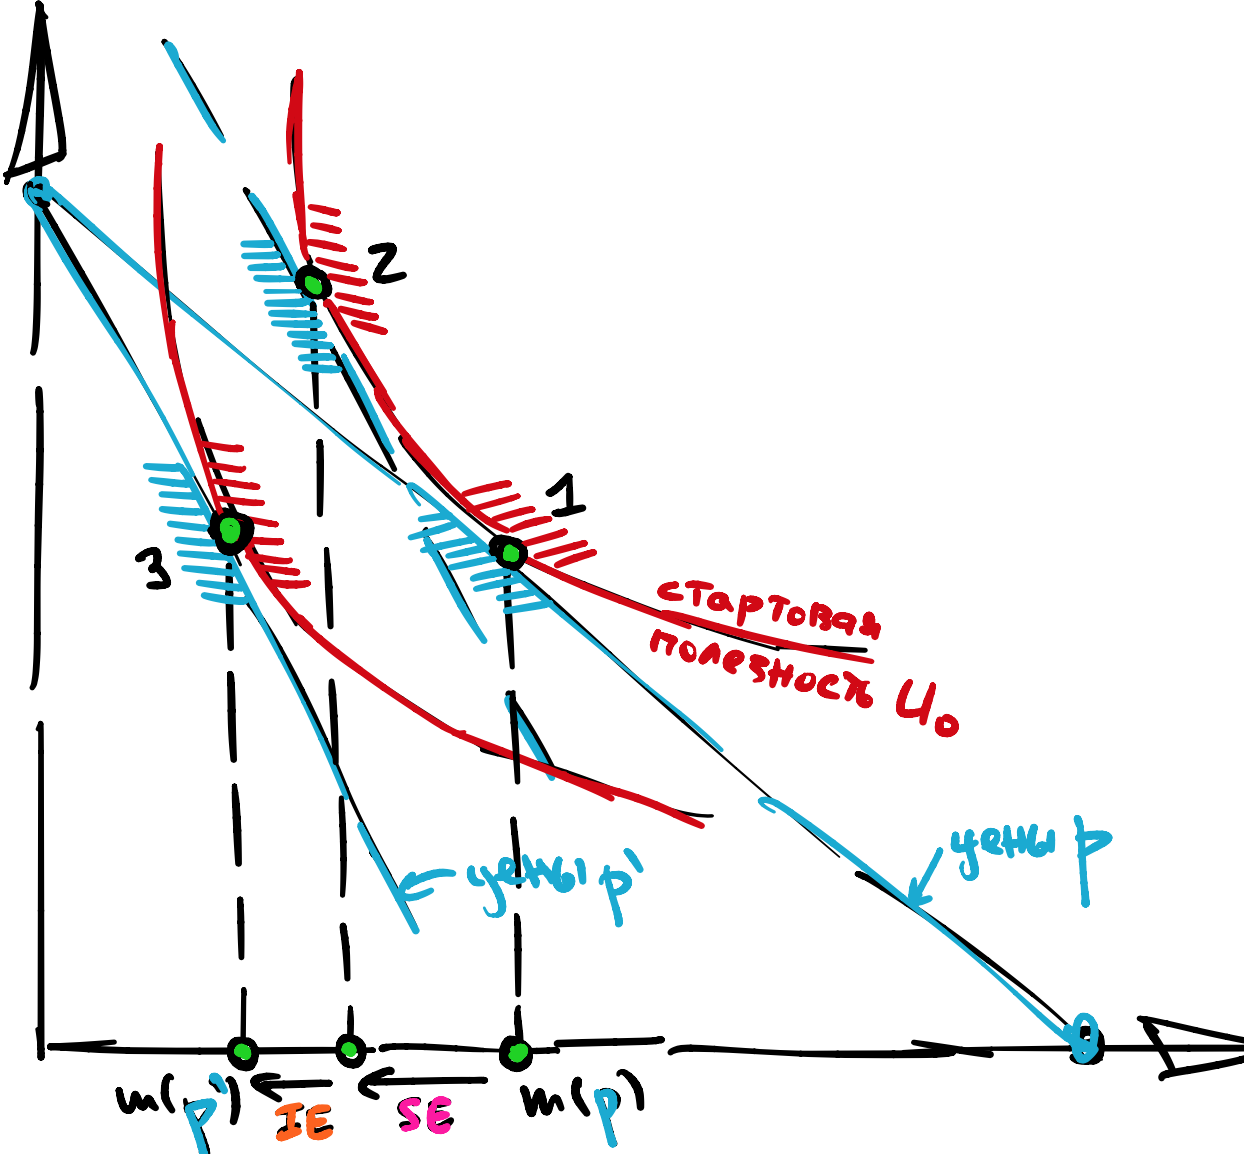
\includegraphics[width=.8 \textwidth]{SEIETE.png}
\end{figure}

\end{frame}

\begin{frame}{Общий эффект}

Есть также общий эффект (TE), он равен сумме эффекта замещения и эффекта дохода и представляет собой просто стандартное изменение маршаллианских спросов:

$$ \text{TE} = \text{SE} + \text{IE} = m(p') - m(p).$$

Поскольку маршаллианский спрос, как правило, наблюдаем, то можно считать, что общий эффект всегда известен. Неизвестно его разложение на эффект дохода и замещения.

\end{frame}

\section{Эффект замещения}

\begin{frame}{Эффект замещения}

Эффект замещения есть, по сути, приращение хиксианского спроса при полезности зафиксированной на изначальном уровне. 
$$ SE = h(p', \bar U_0) - h(p, \bar U_0) $$

Эффект замещения всегда отрицательный (неположительный, если быть точным), если он по своей цене, потому что мы доказали, что $\nabla^2 E \leqslant 0$.

\end{frame}

\begin{frame}{Эффект замещения}

\begin{figure}[hbt]
\centering
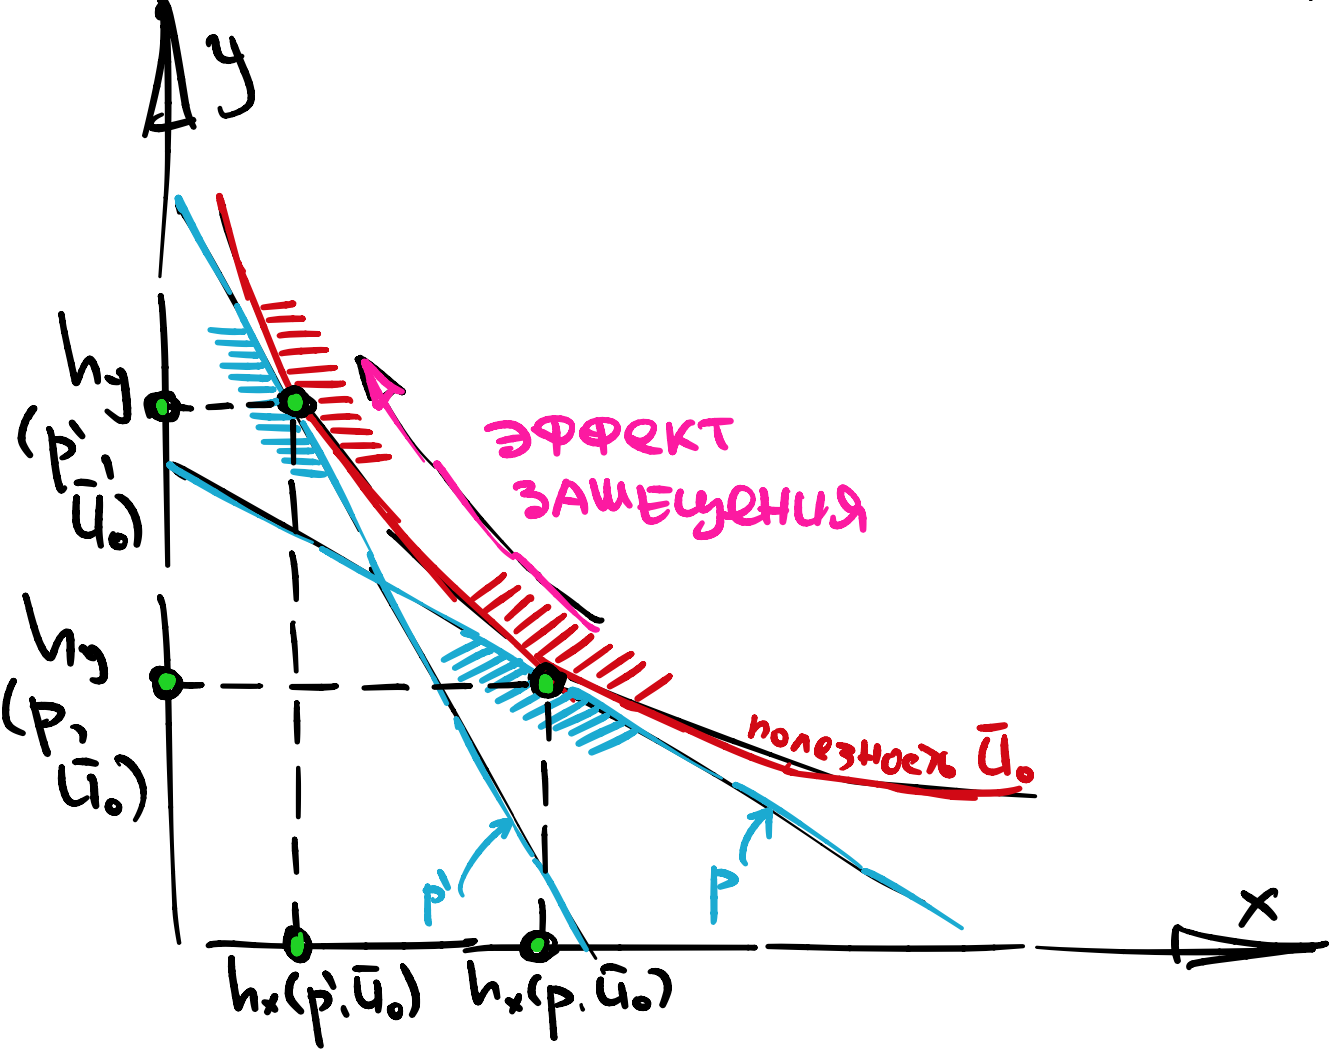
\includegraphics[width=.8 \textwidth]{SE.png}
\end{figure}

\end{frame}

\section{Эффект дохода}

\begin{frame}{Эффект дохода}

Эффект дохода есть разница между общим эффектом и эффектом замещения, именно так его надо считать. 

Однако сам по себе он не представляет большого интереса. Вообще не очень понятно, зачем вычислять кусок спроса, за который отвечает эффект дохода. 

Гораздо интереснее понять, какому изменению бюджета соответствует эффект дохода? Тогда при любом изменении цен, мы можем сказать насколько мы "ограбили" того или иного потребителя в рублях.

Это же как раз компенсирующая вариация $CV$!

\end{frame}

\begin{frame}{Эффект дохода}

\begin{figure}[hbt]
\centering
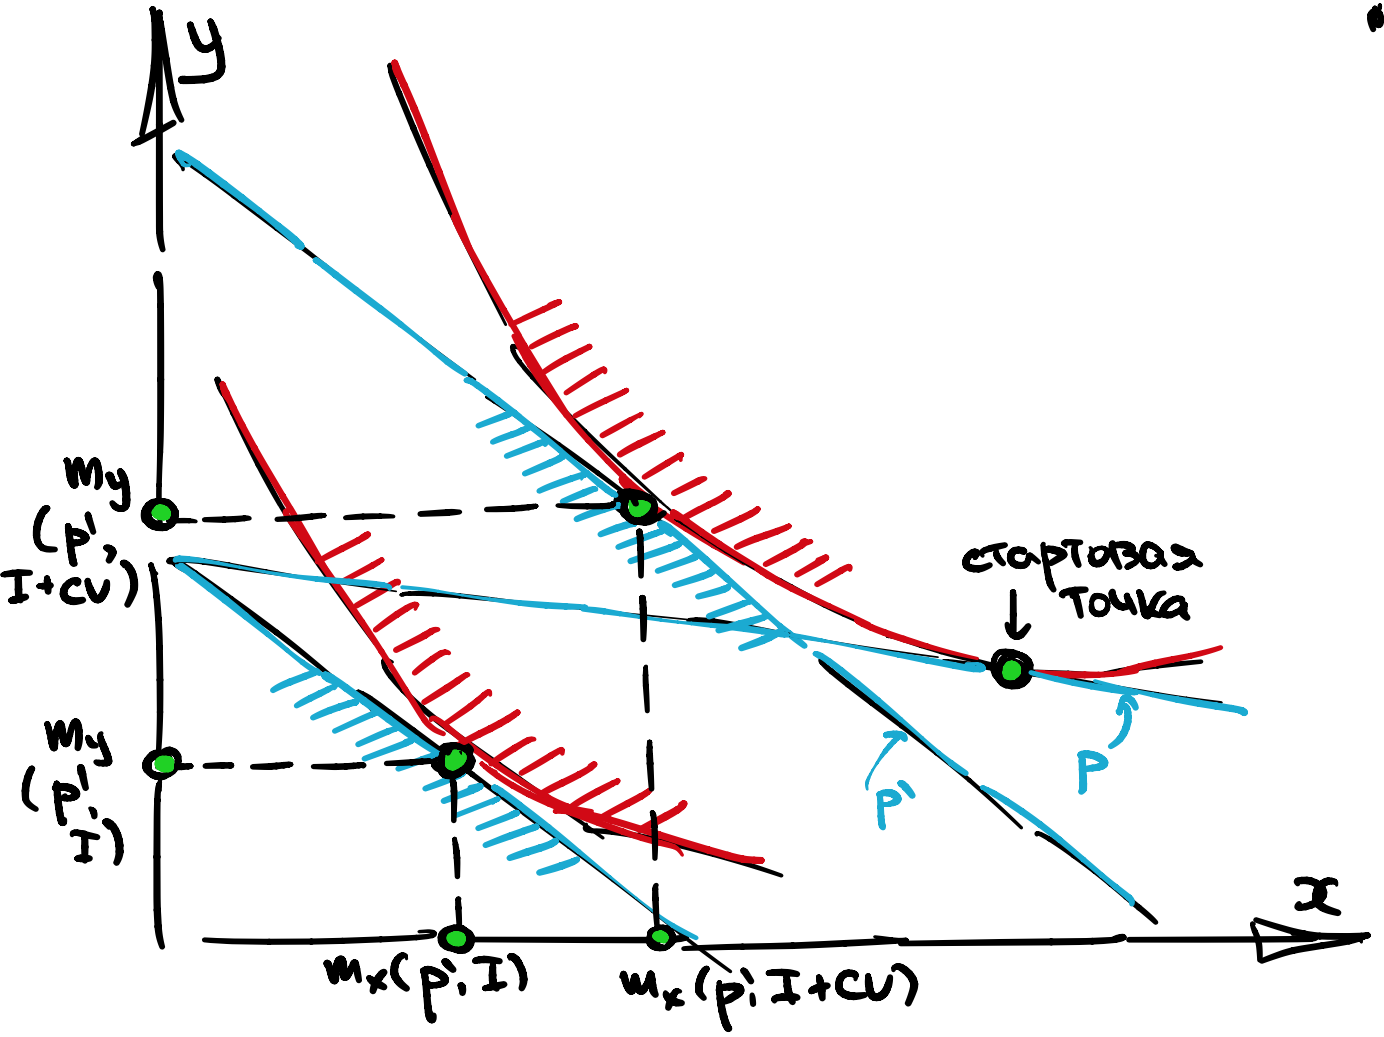
\includegraphics[width=.8 \textwidth]{IE.png}
\end{figure}

\end{frame}

\section{Матрица Слуцкого}

\begin{frame}{Матрица Слуцкого}

Сфокусируемся на уравнении, связывающем Хиксианский и Маршаллианский спросы:
$$\vec h (\vec p, \bar U) = \vec m(\vec p,  E(\vec p, \bar U)).$$
Вас, скорее всего, не учили матричному дифференцированию, но в данном случае оно работает примерно как обычное:
$$ \nabla \vec h(\vec p,  \bar U) = \nabla \vec m(\vec p,  \bar U) + \frac{\partial m}{\partial I} \cdot \nabla E(\vec p, \bar U) = \nabla \vec m(\vec p,  \bar U) + \frac{\partial m}{\partial I} \cdot \vec h $$

\end{frame}

\begin{frame}{Матрица Слуцкого}

Проблема в том, что и $\frac{\partial m}{\partial I}$ и $\vec h$ – это вектора длины $n$, и, поэтому, мы должны подумать, в каком порядке мы их хотим перемножить. 

Есть два варианта: либо мы умножаем строку $\frac{\partial m}{\partial I}$ на столбец $\vec h$, либо мы умножаем столбец $\frac{\partial m}{\partial I}$ на строку $\vec h$. 

Один из этих вариантов даст число, а другой – матрицу. Тот вариант, который сохранит размерность объекта, и будет правильным матричным дифференцированием. 

Однако это еще не все. 

\end{frame}

\begin{frame}{Матрица Слуцкого}

В зависимости от того, что идет по строкам: координаты цен или координаты товаров – формула будет выглядеть по-разному. 

Например, если по горизонтали идут товары, то правильно:
$$ 
(\nabla h_x, \nabla h_y) = (\nabla m_x, \nabla m_y) + 
\begin{pmatrix} 
h_x \\
h_y
\end{pmatrix} 
\cdot (\frac{\partial m_x}{\partial I}, \frac{\partial m_y}{\partial I})
$$

Чтобы не запутаться, достаточно запомнить, что вектор $h$ в правой части уравнения – это, на самом деле $\nabla_{\vec p} E$, то есть он относится к ценам, которые идут по вертикали.

\end{frame}

\begin{frame}{Матрица Слуцкого}

\begin{definition}
Матрица $S = \nabla h$ называется \textbf{матрицей Слуцкого}, или матрицей замещения.
\end{definition}

\begin{lemma}
Если полезность дважды дифференцируема, то матрица Слуцкого симметрична, так как $S = \nabla^2 E$.
\end{lemma}

\end{frame}

\section{Слуцкий в Кобб Дугласе}

\begin{frame}{Матрица Слуцкого}

Есть много способов вывести матрицу Слуцкого для Кобба-Дугласа, но, пожалуй, самый естественный - это сосчитать руками Гессиан функции расходов. Напомним, что
$$ \log E = U + C + \alpha \log p + \beta \log q.$$

Тогда 
$$ \frac{\partial}{\partial p} E = \frac{\alpha}{p} E, \quad \frac{\partial}{\partial q} E = \frac{\beta}{q} E.$$

\end{frame}

\begin{frame}{Матрица Слуцкого}

Дифференцируя второй раз, получаем повторную производную:
$$ \frac{\partial^2}{\partial^2 p} E = \frac{-\alpha}{p^2} E + \frac{\alpha^2}{p^2} E, \quad \frac{\partial^2}{\partial^2 q} E = \frac{-\beta}{q^2} E + \frac{\beta^2}{q^2} E$$

И, конечно, смешанную производную:
$$ \frac{\partial^2}{\partial p \partial q} E = \frac{\alpha \beta}{p q} E.$$

\end{frame}

\begin{frame}{Матрица Слуцкого}

Наконец, можно вывести матрицу Слуцкого:
$$ S = 
E \cdot 
\begin{pmatrix} 
\frac{-\alpha + \alpha^2}{p^2} & \frac{\alpha \beta}{p q} \\
\frac{\alpha \beta}{p q} & \frac{-\beta +\beta^2}{q^2}
\end{pmatrix} = 
E \cdot \alpha \beta \cdot
\begin{pmatrix} 
\frac{-1}{p^2} & \frac{1}{p q} \\
\frac{1}{p q} & \frac{-1}{q^2}
\end{pmatrix}
$$
\end{frame}

\section{Зачем нужны матрицы Слуцкого}

\begin{frame}{Матрица Слуцкого}
Во-первых, матрица Слуцкого – это в некотором смысле четвертая модель поведения потребителя. То есть вместо калибровки полезности или предпочтений, мы можем калибровать матрицу замещения. 

Коэффициенты матрицы Слуцкого можно переписать в терминах эластичности, дохода и долей, каждый из которых достаточно легко оценивается в данных. 
\end{frame}

\begin{frame}{Матрица Слуцкого}

К примеру, если $s_x$ и $s_y$ это доли товаров $x, y$ в бюджете, то верхний диагональный элемент матрицы Слуцкого можно записать как:
$$ \frac{\partial h_x}{\partial p} = \frac{m_x}{p} (\varepsilon_{x,p} + \varepsilon_{x,I} \cdot s_x)$$

А диагональный элемент матрицы Слуцкого можно записать как:
$$ \frac{\partial h_x}{\partial q} = \frac{m_x}{q} (\varepsilon_{x,q} + \varepsilon_{x,I} \cdot s_y)$$

К слову, эти уравнения связывают эластичности хиксианского и маршаллианских спросов. Правда, это совершенно бесполезно.

\end{frame}

\section{SE в первом приближении}

\begin{frame}{SE в первом приближении}

Матрица Слуцкого указывает нам на приращение Хиксианского спроса. 

\begin{lemma}[SE в первом приближении]
$$ SE = h(p') - h(p) = \int_p^{p'} \frac{\partial}{\partial p} h(x) dx \approx (p'-p) \nabla h$$	
\end{lemma}

То есть если матрица оценена хорошо, то можно сказать, что приращение Хиксианского спроса – это приблизительно произведение матрицы Слуцкого на приращение цен. 

А приращение Хиксианского спроса – это и есть $SE$.

\end{frame}

\section{CV во втором приближении}

\begin{frame}{CV во втором приближении}

Компенсированная вариация это приращение функций расходов $E$, то есть это площадь под $\nabla E$. А это в свою очередь примерно площадь трапеции (на боку) с основанием $(p'-p)$ и сторонами $h(p)$ и $h(p')$, см. иллюстрацию:

\end{frame}

\begin{frame}{CV во втором приближении}

\begin{figure}[hbt]
\centering
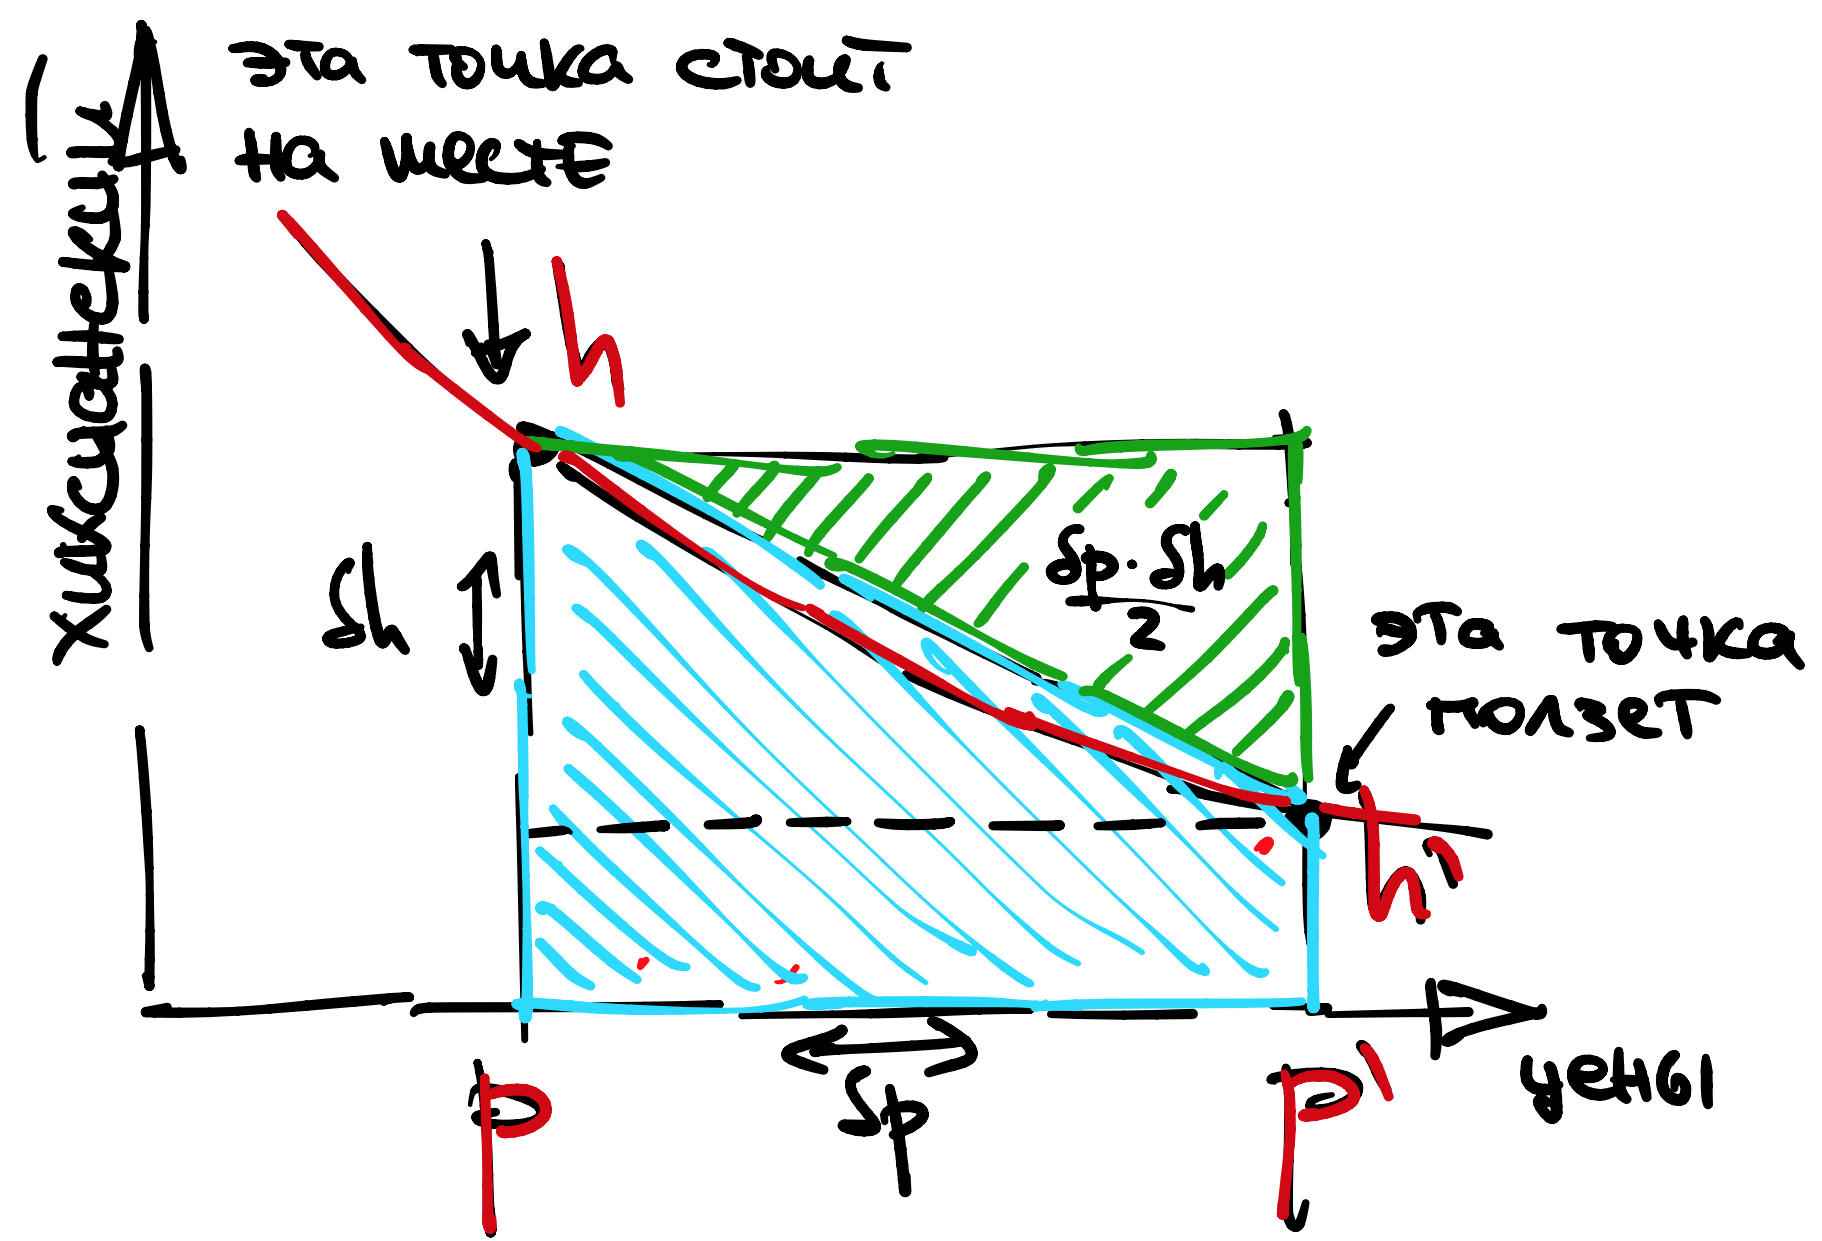
\includegraphics[width=.8 \textwidth]{slutsky.png}
\end{figure}

\end{frame}

\begin{frame}{CV во втором приближении}

Сосчитаем приближенную площадь:

\begin{gather*}
E(p', \bar U) - E(p, \bar U) = \int_p^{p'} h(x, \bar U) dx \approx\\
\approx \frac{(p'-p)(h(p')+h(p))}{2}\\
 = (p'-p)(\frac{h(p') - h(p)}{2} + h(p))
\end{gather*}

\end{frame}

\begin{frame}{CV во втором приближении}
Мы только что доказали достаточно полезное на практике свойство:

\begin{lemma}[CV во втором приближении]
Компенсирующую (но не эквивалентную) вариацию можно приблизить как:
$$CV \approx \delta p \cdot \vec h - \frac{\delta p \cdot S \cdot \delta p^T}{2}$$
при малых $\delta p = p' - p$, где $\vec h$ - действующий спрос.
\end{lemma}

Сравните ответ с разложением $CV$ для Кобба-Дугласа, которую мы вывели раньше.

\end{frame}

\section{Парадокс Гиффена}

\begin{frame}

Парадокс Гиффена заключается в том, что для некоторых товаров, которые пользовались популярностью у бедных: картофель и дешевый хлеб – наблюдалась прямая зависимость между ценой и спросом. Похожая зависимость иногда прослеживается для спроса на рис в современном Китае.

Разрешение парадокса осуществляется за счет анализа Хиксианского спроса и матриц Слуцкого. 

\end{frame}

\begin{frame}

Обратим внимание еще раз на эластичность Хиксианского спроса по собственной цене, которую я назову $\varepsilon^c_{x,p}$:
$$\varepsilon^c_{x,p} = \varepsilon_{x,p} + \varepsilon_{x,I} \cdot s_{x},$$

и перепишем ее так, чтобы маршаллианский спрос был слева:
$$\varepsilon_{x,p} = \varepsilon^c_{x,p} - \varepsilon_{x,I} \cdot s_{x}.$$

Легко видеть, что если $\varepsilon_{x,I} > 0$, то, поскольку $\varepsilon^c_{x,p}$ всегда неположительный, и $\varepsilon_{x,p}$ будет неположительный. А нам нужна положительная зависимость между $x,p$. 
\end{frame}

\begin{frame}

Соответственно, можно сделать следующий вывод:

\textbf{Нормальный товар не объяснит парадокс Гиффена.}

\end{frame}

\begin{frame}

Соответственно, можно сделать следующий вывод:

\textbf{Нормальный товар не объяснит парадокс Гиффена.}

\end{frame}

\begin{frame}
Предположим, наоборот, что товар $x$ инфериорный, то есть это товар низкого качества, тогда $\varepsilon_{x,I} < 0$. Предположим также, что доля товара $x$ в бюджете потребителя достаточно высока, то есть $s_{x}$ большой. Наконец, предположим, что для товара $x$ нет близкого (чистого) субститута, то есть $\varepsilon^c_{x,p}$ близок к нулю.

Тогда может так случиться, что $\varepsilon_{x,p}$ станет положительным.

\end{frame}

\begin{frame}
Еще раз
$$\varepsilon_{x,p} = \varepsilon^c_{x,p} - \varepsilon_{x,I} \cdot s_{x}.$$

\begin{itemize}
\item $\varepsilon^c_{x,p}$ называется эффектом замещения
\item $\varepsilon_{x,I} \cdot s_{x}$ называется эффектом дохода
\end{itemize}

Для того, чтобы объяснить парадокс Гиффена, нужно иметь слабый эффект замещения и сильный отрицательный эффект дохода.

\end{frame}

\begin{frame}
\begin{figure}[hbt]
\centering
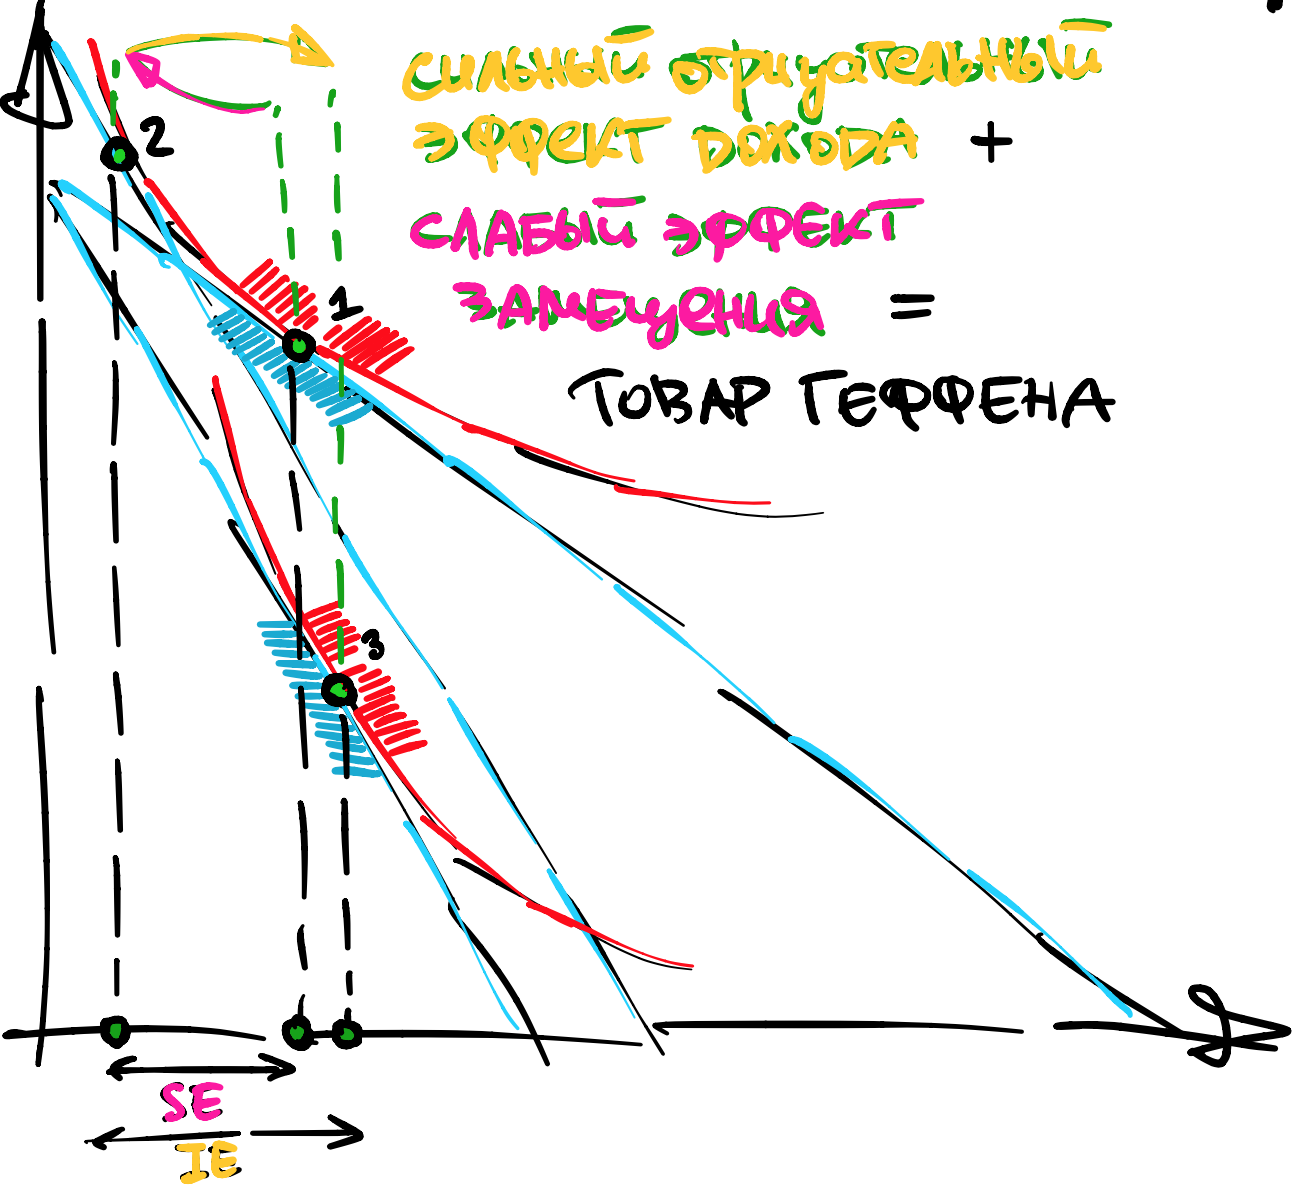
\includegraphics[width=.8 \textwidth]{IESE_CV.png}
\end{figure}

\end{frame}

\section{Это была самая сложная лекция}

\end{document}